\documentclass[12pt]{jarticle}
\usepackage[dvipdfmx]{graphicx}
\usepackage{amsmath}
\usepackage{amsthm}
\usepackage{listings, jlisting}
\usepackage{multirow}

\setlength{\topmargin}{30mm}
\addtolength{\topmargin}{-1in}
\setlength{\oddsidemargin}{20mm}
\addtolength{\oddsidemargin}{-1in}
\setlength{\evensidemargin}{20mm}
\addtolength{\evensidemargin}{-1in}
\setlength{\textwidth}{170mm}
\setlength{\textheight}{245mm}
\setlength{\headsep}{0mm}
\setlength{\headheight}{0mm}
\setlength{\topskip}{0mm}

%定義とか
\newtheorem{theorem}{定理}[section]
\newtheorem{definittion}{定義}[section]

% ソースコード貼付け用の設定
% \usepackage{caption}
% \captionsetup[lstlisting]{font={small,tt}}
\lstset{%
  language={Python},
  basicstyle={\small},%
  identifierstyle={\small},%
  commentstyle={\small\itshape},%
  keywordstyle={\small\bfseries},%
  ndkeywordstyle={\small},%
  stringstyle={\small\ttfamily},
  frame={tb},
  breaklines=true,
  columns=[l]{fullflexible},%
  numbers=left,%
  xrightmargin=0zw,%
  xleftmargin=3zw,%
  numberstyle={\scriptsize},%
  stepnumber=1,
  numbersep=1zw,%
  lineskip=-0.5ex%
}

\begin{document}

\pagestyle{empty}
\begin{center}
  \vspace*{3.0cm}
  {\fontsize{80pt}{100pt}\selectfont 卒業論文}

  \vspace*{2.0cm}

  \begin{LARGE}
    Twitterを用いた新聞記事への\\
    自動ソーシャルアノテーションツールに関する研究
    \vspace*{2.0cm}

    平成 26 年 2 月 7 日提出
  \end{LARGE}

\end{center}
\begin{LARGE}
  \vspace*{1.0cm}
  \hspace{25mm}指導教員\hspace{51mm}伊庭斉志\,教授

  \hspace{70mm}ダヌシカ ボレガラ\,講師

  \vspace*{1.0cm}
  \begin{center}
    電子情報工学科

    \vspace{1.0cm}
    03-120443\hspace{15mm}村上\,晋太郎
  \end{center}

\end{LARGE}

\newpage
\tableofcontents

\newpage
\setcounter{page}{1}
\pagestyle{plain}

\section{序論}
\subsection{背景}
2000年代後半から, Facebook, Twitter, Google+などのソーシャルネットワーキングサービスが盛んに利用されるようになった. 2012年には, Facebookのアクティブユーザ数は10億人\footnote{http://ja.wikipedia.org/wiki/Facebook}を突破し, Twitterでもアクティブユーザー数は1.4億人\footnote{http://www.724685.com/twitter/tw13050310.htm}となっている. Facebookでは一日当たり0.5ペタバイトのデータが増加しており, Twitterへの投稿数は一日当たり3.4億投稿となっている.
このように, ソーシャルネットワーキングサービスは利用者数の面でも, データ量の面でも莫大な資源となっており, 様々な利用が期待される.

一方, 近年インターネット上で閲覧することが出来るニュース記事が増加している. 日本では, 朝日新聞社\footnote{http://www.asahi.com}, 読売新聞社\footnote{http://www.yomiuri.co.jp}, 毎日新聞\footnote{http://mainichi.jp}等の大手新聞者がインターネット上でニュース記事を配信している. 海外でも, Washington Post\footnote{http://www.washingtonpost.com} Los Angels Times\footnote{http://articles.latimes.com}等, 大手新聞社が同様のサービスを提供している.

ソーシャルネットワーキングサービスの書き込みの中には, このようなインターネット上のニュース記事に言及しているものが多数存在する. このような書き込みには, 一般のインターネットユーザーの個人的な意見, 見解が記されている. このようなインターネット上のニュース記事と, ソーシャルネットワーキングサービスへの書き込みを結びつけることで, 報道機関のプロの書き手とソーシャルネットワーキングサービス上で活動する一般社会の書き手を結びつけることができるようになる. このようなツールが実現すれば, 報道機関のプロの書き手は自分の書いた記事が一般社会にどのような影響を与えているのかについての情報を, より簡単に得る事が出来るようになる. 一方, 一般の書き手にとっては, ニュース記事に情報が付与されるようになり専門的な内容の記事を読みやすくなったり, ニュース記事からより有用な情報を引き出せるようになる.

また, ニュース記事を学術論文に, ソーシャルネットワーキングサービス上の投稿を学術論文に対するコメントに置き換えた場合も, 同じ手法を用いることができ, その場合にも同じ効果が期待できるという点で, 応用性も高いと考える.

以上のような背景から, 本研究ではソーシャルネットワーキング上の情報とインターネット上のニュースを自然言語処理の手法を用いて結びつけることを目標とする.

\clearpage

\subsection{目的}
本研究では, ソーシャルネットワーキングサービス「Twitter」上の投稿をインターネット上のニュース記事に自動付与(アノテーション)するツールを作成することを目的とする. 本研究に置けるツールでは, ニュース記事単位をTwitter上の投稿の付与の対象とするのではなく, ニュース記事の中の文単位を付与の対象とする(図\ref{fig1}). 結果, ユーザはニュース中のどの部分に対して, Twitter上でどのような反応が起こっているのかが分かるようになる. このようなツールが実現すれば, ニュース記者にとってはは自分の書いた記事についてのユーザーの意見が簡単に見れるようになり, フィードバックをすぐに得る事ができるようになるという点で有用である. 一方, 読者にとっては, 難しい内容のニュース記事でも他のユーザーによる情報付与があることにより, 理解の助けとすることができる. Twitter上の投稿をWeb上のニュース自体に結びつけるタスクは, 先行研究で既に取り扱われているが, Twitter上の投稿をWeb上のニュースの中の断片に結びつけるというタスクはまだ取り扱われていない. その点が, 本研究の新規性である.

\begin{figure}[htbp]
  \begin{center}
    \includegraphics{ai/social_annotation.eps}
  \end{center}
  \caption{Twitterを用いたソーシャルアノテーションツール}
  \label{fig1}
\end{figure}

本研究ではTwitterとインターネット上のニュース記事を対象にツールの構築を進めていくが, その本質は「大きな文章中のセンテンスの集合と, 小さな文章の集合のアラインメント」である. そのため, 「背景」でも述べたように, 本研究で得られた成果を, Twitterやインターネット上のニュース記事に限らずに応用することが可能である. 例えば, ニュースを学術論文に置き換え, Twitter上の投稿をその論文に対するレビューに置き換えることで, その学術論文のどの部分にどのような反応が起きているかを知る事が出来るツールを構築可能である.

\newpage

\section{手法}
本研究では, ニュース上の記事の断片に対して, ソーシャルネットワーキングサービス「Twitter」上の投稿から関連度の高いものを結びつけるツールを作成する. この章では, そこで用いる手法について説明する.

本研究のタスクは, 以下のようなステップに分けることができる.

\begin{enumerate}
  \item 記事と関連するニュース記事の収集\\
    Twitter上の投稿の中から, 対象のニュース記事と関連性が高いと思われるものを抽出して収集する.
  \item 内容語の抽出\\
    Twitter上の投稿の文中から, Twitter上の投稿とニュース断片の関連度の計算にほとんど影響しないと判断できる単語を除去する.
  \item 関連度の計算\\
    Twitter上の投稿と, ニュースの断片との関連度を計算して数値化する.
  \item ニュース断片とTwitter上の投稿の結びつけ\\
    計算されたTwitter上の投稿とニュース断片の関連度をもとに, ニュース断片へのTwitter上の投稿の結びつけを行う.
\end{enumerate}

以下で, 上記のそれぞれのステップについて詳しく説明をする.

\subsection{記事と関連するニュース記事の収集}
記事と関連するニュースの収集に関しては, 同じタスクを取り扱った先行研究がすでにあるため本研究では深く取り扱わない. 以下, 本研究における暫定的な手法について説明する.

Twitter上においては, あるニュースに関する投稿をする際に, そのニュースのタイトルを併記するという慣習がある. そこで, 本研究では, 対象のニュースのタイトルを含むTwitter上の投稿を, その記事と関連するニュースとして自動的に収集するようにした. しかし, Twitter上の投稿の中には,

\begin{itemize}
  \item タイトルを併記せずにそのニュースに言及しているもの
  \item 誤植などで不完全な形でタイトルを併記してそのニュースに言及しているもの
  \item そのニュースに言及はしていないが, 偶然タイトルを含んでいるもの
\end{itemize}
が存在する. また, 他のソーシャルネットワーキングサービス上で同様の慣習が根付いているとは限らないため, 応用の範囲も狭められる. 今後先行研究をもとに記事の収集を別の手法に置き換えることが望ましいと考える. これについては今後の課題としたい.

\subsection{内容語の抽出}
自然言語の文の特性を調べる際に, bag-of-words\cite{nlpml}という考え方がる. bag-of-wordsでは, ある文の特性を解析する際に, その文にどのような単語がどのくらい含まれているのかを計算して, それをもとに文の特性を解析し, クラスタリング等のタスクを行う. 本研究でも, webニュースの断片に含まれる単語と, Tweetに含まれる単語の集合を比較して, webニュースの断片とTweetの関連度を計算する.

一般に, 自然言語の文中には, その文章の持つ素性を計算する際にほとんど情報をもたないような単語が多く含まれる. 副詞や格助詞などがそうである. 反対に, その文章の持つ素性を計算する際に有用な情報を与える単語を内容語と定義する. 非内容語である単語をあらかじめ除去し, 内容語を抽出しておくことで, 関連度の計算の精度を高めることが出来ると考えられる. 関連度の計算の前処理として, この内容語の抽出を行う.

内容語の抽出には, 二通りの方法が考えられる. 一つ目は, 形態素解析ツールを使用し, 単語の品詞を分析した上で, 副詞や格助詞などの非内容語であると考えられる単語を除去する方法である. 二つ目は, 統計的な手法を用いて, その単語のその文章における重要度を計算し, 一定の重要度以下の値を持つ単語を非内用語として除去する方法である.

一つ目の方法は比較的簡単に実現でき, 一定の精度も期待できるが,
\begin{itemize}
  \item 形態素解析ツールに依存するため他言語に拡張できない
  \item ソーシャルネットワーキングサービス特有の, ネットスラングなどの語彙に対応できない
\end{itemize}
といった問題点が存在する. そこで, 本研究では二つ目の, 統計的手法を採用する.

\subsubsection{tf-idf}
本研究では, 統計学的手法としてtf-idf\cite{tfidf}を採用する. tf-idfは, 文書中である単語が, その文章をどの程度特徴づけているかの重み度合いである. tf-ifdは, 以下の式によって定義される.

\begin{equation}
  \rm{tfidf}_{w,d} = \rm{tf}_{w,d} \cdot \rm{idf}_{w}
\end{equation}

\begin{equation}
  \rm{tf}_{w, d} = \frac{n_{w,d}}{\sum_k n_{w,d}}
\end{equation}

\begin{equation}
  \rm{idf}_{w} = \log{\frac{|D|}{|\{d|t_w \in d\}|}}
\end{equation}

ここで, $n_{w,d}$は単語$w$の文書$d$における出現回数, $|D|$は総ドキュメント数, $|\{d|t_w \in d\}|$は単語$w$を含む総ドキュメント数である.

この式の意味するところは, 「どのような文書にも普遍的に出現するような単語の重みは低くなる」ということと, 「ある文書中で頻繁に言及されるような単語があれば, その文書中でのその単語の重みは高くなる」ということである.

本研究では, tf-idfの高い単語は内容語であると判断し, tf-idfの低い単語は内容語では無いと判断する.

本研究では, まず新聞記事を100件以上集め, idfの計算を行う. ここで, 収集する記事が多ければ多いほどidfの精度は上がる. このifdをもとに, webニュースの断片とtweetの関連度を計算する際にtf-idfを計算し, 単語をtf-idfでソートする. そして, その中で閾値以上の単語を内容語とする. この閾値を調整すると, 内容語の数と質が変わるので, 実験によって調整する.

\subsection{関連度の計算}
内容語の抽出を行ったのちに, Twitter上の投稿とニュース断片の関連度の計算を行う. 関連度の計算にも, bag-of-wordsの考え方を採用し, 文中に含まれる単語を分析する.

単語をもとにニュース断片とTwitter上の投稿の関連度を計算する際の指標として, 以下の三つが挙げられる.

\begin{enumerate}
 \item 完全に一致する単語\\
    webニュースの断片とTwitter上の投稿の間に完全に一致する単語がある場合, そのセンテンスとTweetの関連度は高いと考えられる. 図\ref{fig1}の例では, @Maryというユーザーが投稿したtweetに「サウスカロライナ」という単語が含まれているので, 同じ単語を含む一つ目のセンテンスとの関連度が高くなる.
 \item 言い換えの単語\\
    webニュースの断片とTwitter上の投稿に言い換えの関係にある単語が含まれている場合, そのセンテンスとTweetの関連度は高くなると考えられる. 図\ref{fig1}の例では, @Davidというユーザーが投稿したtweetに「米国」と言い換えの関係にある「アメリカ」という単語が含まれているので, 「米国」という単語が含まれる, 5行目から始まるセンテンスとの関連度が高くなる.
 \item 互いに類似する単語\\
    webニュースの断片とtweetの文に, 同じ文脈で使われるような単語が含まれている場合, そのセンテンスとTweetの関連度は高くなると考えられる. 図\ref{fig1}の例では, @Tomというユーザーが投稿したTweetに「早死に」という単語が含まれており, これは「死亡率」という単語と同じ文脈で使われる単語であると判断できるので, 一行目から始まるセンテンスとの関連度が高くなる.
\end{enumerate}

これらの単語が含まれていたら値が高くなるようにセンテンスとTweetの関連度を定義する. このようにすることで, ニュースwebニュースの断片とTwitter上の単語を比較し, のアラインメントをとることができる.

上記の完全に一致する単語, 言い換えの単語, 互いに類似する単語の中でも, 単語によってニュース記事とTwitter上の投稿の関連度に対する影響は異なると考えられる. そこで, 本研究ではこの影響の違いをtf-idfで重み付けすることで対応する. また, 「一致する単語」, 「言い換えの単語」, 「互いに類似する単語」の三つの集団でも, ニュース記事とTwitter上の投稿の関連度に対する影響は異なると考えられる. これは定数で重み付けをすることで対応する. この定数は, 実験で調整する.

以上より, Tweet$t$とニュース断片$s$の関連度を以下の式によって定義する.

\begin{equation}
  {\rm Rel}(s, t) = \alpha \sum_{\{w|w \in A\}} w * {\rm tfidf}_{w, d} +
                    \beta  \sum_{\{w|w \in B\}} w * {\rm tfidf}_{w, d} +
                    \gamma \sum_{\{w|w \in C\}} w * {\rm tfidf}_{w, d}
  \label{eq:rel}
\end{equation}

ここで, $A$は$s$と$t$の中で完全に一致する単語の集合であり, $B$は$s$と$t$の中で言い換えの関係にある単語の集合であり, $C$は$s$と$t$の中で互いに類似の関係にある単語の集合である. 同じ単語が複数回出てきた場合も, それは別々の単語として処理する. すなわち, tf-idfの高い単語が$s$と$t$の両方に複数回にわたって出現していたら, それだけ関連度${\rm Rel}(s, t)$は高くなる. $\alpha$, $\beta$, $\gamma$は定数であり, 実験によりアラインメントの結果を見ながら調整する. 「完全に一致する単語」の方が, 「言い換えの単語」や「互いに類似する単語」よりも関連度に大きな影響力を持つと考えられる. また, 「言い換えの単語」は「互いに類似する単語」よりも関連度に大きな影響力を持つと考えられる. そのため, $\alpha > \beta > \gamma$となることが予想される.

上記であげた蜜の集合のうち, $A$の「完全に一致する単語」は容易に発見することができる. それに対して, $B$の「言い換えの単語」や, $C$の「互いに類似する単語」を識別するためには, 統計的な処理が必要となる. この手法については後述する.

\subsubsection{言い換えの関係の語の検出}
本研究では「言い換えの単語」の検出方法として, WordNet\footnote{http://nlpwww.nict.go.jp/wn-ja/}を利用する. WordNetは, 英語の概念辞書である. WordNetでは, 単語がsynsetという同義語のグループにまとめられている. よって, 同一のsynsetに含まれる単語は言い換えの単語であると判断できる. WordNetには英語版の他にも, 独立行政法人情報通信研究機構(NICT)によって日本語版の物が提供されている. また, Python等のプログラミング言語向けのフロントエンドも提供されており, プログラムから動的にデータ資源にアクセスすることが可能である.

\subsubsection{互いに類似する語の検出}
「互いに類似する単語」の検出にはいくつかの方法が考えられるが, 本研究では言い換えの関係の語の検出と同じく, WordNetを利用して類似する単語の検出を行う. しかし, WordNetを用いた類似語の検出にはいくつかの問題点が存在するため, 考えられる代替案としてLinの手法\cite{DekangLin}, Latent Spaceでのモデル化\cite{LatentSpace}, Co Clustering\cite{CoClustering}を後に紹介する.

\clearpage
\subsubsection{WordNetを用いた類似語の検出}
WordNetでは同義語同士がSynsetというグループにまとめられているが, 各々のSynsetは他のSynsetと繋がりを持っている. Synset同士の繋がりにはいくつかの種類がある. Synset同士の繋がりの種類は, 単語の品詞によって異なる. 以下に, 名詞のSynsetにおけるSynset間の繋がりの例を示す.

\begin{itemize}
\item 上位語 \\
すべてのXがYの種類の一であるならYはXの上位語である.
\item 下位語 \\
すべてのYがXの種類の一であるならYはXの下位語である.
\item 同族後 \\
XとYの上位語が同じなら, YはXの同族語である.
\item 全体語\\
XがYの一部であるなら, YはXの全体語である.
\item 部分語 \\
YがXの一部であるなら, YはXの部分語である.
\end{itemize}

以上のような繋がりを用いて, WordNet中ではSynset同士が階層構造を形成している.
Synsetのネットワークの例を図\ref{word_net}に示す.

\begin{figure}[htbp]
  \begin{center}
    \includegraphics[scale=0.5]{image/wordnet.eps}
  \end{center}
  \caption{WordNetにおけるSynset同士の繋がりの例}
  \label{word_net}
\end{figure}

図\ref{word_net}において, artefactはmotor vehicleの上位語であり, motorcar, go-kart, truckはともにmotor vehicleの下位語であるので, 互いに同族語である.

このようなネットワーク上では, 意味の近い単語ほど短い経路でたどり着くことができ, 意味の遠い単語ほどたどり着くのに長い経路を必要とすると考えることができる. このネットワーク上での距離を測定することで, Synset間の類似度を測定することが出来る\cite{wordnet-similarity}. 本研究ではこの性質を利用して単語間の類似度を測定する. そして, 類似度が一定の閾値以上の単語同士を互いに類似する単語として集計する. この類似度は実験により調整する.

\subsubsection{Linの手法の利用}
WordNetによる類似度の測定は効果的であるが, 人手によって構築された意味辞書に依存しているという欠点がある. 英語圏には既に完成度が高いWordNetが存在するが, それをもとに作られた日本語圏のWordNetはまだ語彙数が少ない. このように, WordNetを用いた類似語の検出は言語に依存してしまう. また, ソーシャルネットワーキングサービス上ではネットスラング等の辞書上に無い新しい語彙が用いられる場合もあり, その場合もWordNetでは対応することが出来ない.

以上のような理由から, 本研究のツールにおける類似語の検出には意味辞書に依存せずに, 収集したテキストコーパスから学習できるような手法が望ましいと考えられる.

このような「互いに類似する語」の検出方法として, Linの手法\cite{DekangLin}の利用が挙げられる. これは, 単語同士がどれだけ「似ているのか」を計算するための手法である. Linの手法では, 単語同士の類似度は以下の式で定義される.

\begin{equation}
  {\rm sim}(w_1, w_2) = \frac{\sum_{(r,w)\in T(w_1)\cap T(w_2)} (I(w_1, r, w) + I(w_2, r, w))}{\sum_{(r,w) \in T(w_1)}I(w_1, r, w) + \sum_{(r,w) \in T(w_2)}I(w_2, r, w)}
\end{equation}

ここで, $I$は相互情報量であり, 以下の式で定義される.

\begin{align}
I(w, r, w') & = -\log(P_{MLE}(B)P_{MLE}(A|B)P_{MLE}(C|B))-(-\log P_{MLE}(A,B,C)) \\
 & = \log \frac{||w,r,w||\times||*,r,*||}{||w,r,*||\times||*,r,w'||}
\end{align}

ここで, $||w, r, w'||$という記法は, 単語$w$, $w'$, 単語間の関係$r$に対して$w$が$w'$の$r$であるという関係$(w, r, w')$が成り立つ箇所の総数である. 例えば, "I have a brown dog"という文章では, $w$を"dog", $w'$を"have", $r$を"object of"として, $\rm (dog, objectof, have)$という関係が成り立っているので, $\rm||dog, object of, have||=1$となる.
$w$, $w'$は$*$(ワイルドカード)で置き換えられることもあり, その場合, $*$に全ての単語をあてはめた総数が$||w, r, w'||$の値となる.

$P_{MLE}$は最尤法に基づいて計算される確率であり, $P_{MLE}$の引数となっている$A$, $B$, $C$はそれぞれ以下のような事象である.

\begin{description}
  \item[$A$:]無作為に選出した語が$w$である
  \item[$B$:]無作為に選出した関係が$r$である
  \item[$C$:]無作為に選出した語が$w'$である
\end{description}

$P_{MLE}$は以下の式を満たすことが示されている.

\begin{align}
  P_{MLE}(B)   & = \frac{||*, r, *||}{||*, *, *||}\\
  P_{MLE}(A|B) & = \frac{||w, r, *||}{||*, r, *||}\\
  P_{MLE}(C|B) & = \frac{||*, r,w'||}{||*, r, *||}
\end{align}

これらの定義の意味するところは, 同じ単語と同じ関係にある二つの単語は, 似ている単語であるということである. 例えば, 「車」と「電車」は共に「乗る」という動詞の目的語になるので, 似ている単語と見なすことができる.

本研究では, この定義に従って${\rm sim}(w_1, w_2)$を計算し, この値が閾値を越えたペアを互いに類似する単語とみなす. この閾値を調整すると, 検出される類似語のペアの質が変わるので, 実験によって最適な値を求める.

\subsubsection{Latent Spaceでのモデル化}
意味辞書に依存せずに「互いに類似する語」のもう一つの検出方法としてLatent Spaceでのセンテンスのモデル化\cite{LatentSpace}が挙げられる. この手法では,

\begin{equation}
  X_{ij} = {\rm tfidf}_{i,j}
\end{equation}

によって定義される$M \times N$行列$X$を, $M \times K$行列$P$, $N \times K$行列$Q$を用いて

\begin{equation}
  X \approx P^T Q
\end{equation}

と近似的に分解することにより, 次元数の低い素性を抽出する手法である. ここで, $P$, $Q$はランダムに初期化された上で

\begin{align}
  P_{\cdot ,i} &= (Q\tilde W^{(i)}Q^T + \lambda I)^{-1} Q \tilde W^{(i)} X_{i, \cdot }^T \\
  Q_{\cdot ,i} &= (P\tilde W^{(j)}P^T + \lambda I)^{-1} P \tilde W^{(i)} X_{\cdot , j}^T
\end{align}

によって段階的に求められる. $W^{(i)}$は,
\begin{displaymath}
W_{i,j} = \left\{
\begin{array}{l}
1\;\;\;\;\;{\rm if} \;\; X_ij \neq 0 \\
w_m\;\;\;{\rm if} \;\; X_ij = 0
\end{array}
\right.
\end{displaymath}

によって定義される$W$のi行目を成分とする対角行列で,

\begin{equation}
  W^{(i)} = {\rm diag}(W_{\cdot, i})
\end{equation}
と表される.

行列Pの各列には, Xに現れていた, 各単語の「どの文書でどのくらい重要になるか」という特徴量が低次元に圧縮されて格納されている. これは, 単語の情報が抽象化されて入っていると言える. このPの中で, コサイン類似度の高い列同士のペアを見つければ, その列に割り当てられている単語同士は互いに類似する単語と言えるようになる. 本研究では, コサイン類似度が閾値を越えたペアを類似語とみなす. この閾値を調整すると, 検出される類似語のペアの質が変わるので, 実験によって最適な値を求める必要がある.

\subsection{ニュース断片とTwitter上の投稿の結びつけ}
この段階では, 式\ref{eq:rel}により算出されたwebニュース断片とTwitter上の投稿の関連度をもとに, ニュース断片とTwitter上の投稿の結びつけを行う. これを, アラインメントと定義する. ニュース断片とTwitter上の投稿の結びつけでは, 全てのTwitter上の投稿がニュース断片と結びつくような状態になってはいけない. 逆に, 全てのTwitter上の投稿がニュース断片に結びつかないような状態になっても, ツールとしての有効性が失われる. したがって, この段階ではTwitter上の投稿がニュース断片にほどよくばらけて結びつくようにコントロールする必要がある. 本研究では, このようなことが実現可能な手法として, 安定結婚アルゴリズム\cite{smp}の拡張である, 一対多の安定結婚アルゴリズム\cite{psmp}によるアラインメントを採用した.

\subsubsection{安定結婚問題}
この節では安定結婚問題の概要とその解法を説明する.

安定結婚問題\cite{smp}は, 安定マッチング問題の一つである.
安定結婚問題では, N人の男性とN人の女性がいる状況で, 「不倫」の起こることの無いようにN組の結婚を成立させることを目的とする.
不倫の起こらないN組の結婚の組み合わせを, 「安定なマッチング」という.
安定結婚問題では, N人の男性はそれぞれ, どの女性を好むかを順位付けした長さNの選好度リストをもっている.
N人の女性もそれぞれ同様に, どの男性を好むかを順位付けした長さNの選好度リストを持っている.
ここでいう「不倫」とは, N組のカップルが成立している中で, 互いに現在組んでいるカップルよりも好きなペアが発生することを指す.
このようなペアを「ブロッキングペア」と定義する.

安定結婚問題の例を図\ref{match}に示す. 図\ref{match}上段の安定なマッチングの例では, ブロッキングペアが存在しないので不倫は起こらない.
それに対して, 図\ref{match}下段の不安点なマッチングの例では, 男性4と女性4のペアがブロッキングペアとなるので, 不倫がおこってしまう.

\begin{figure}
  \begin{center}
    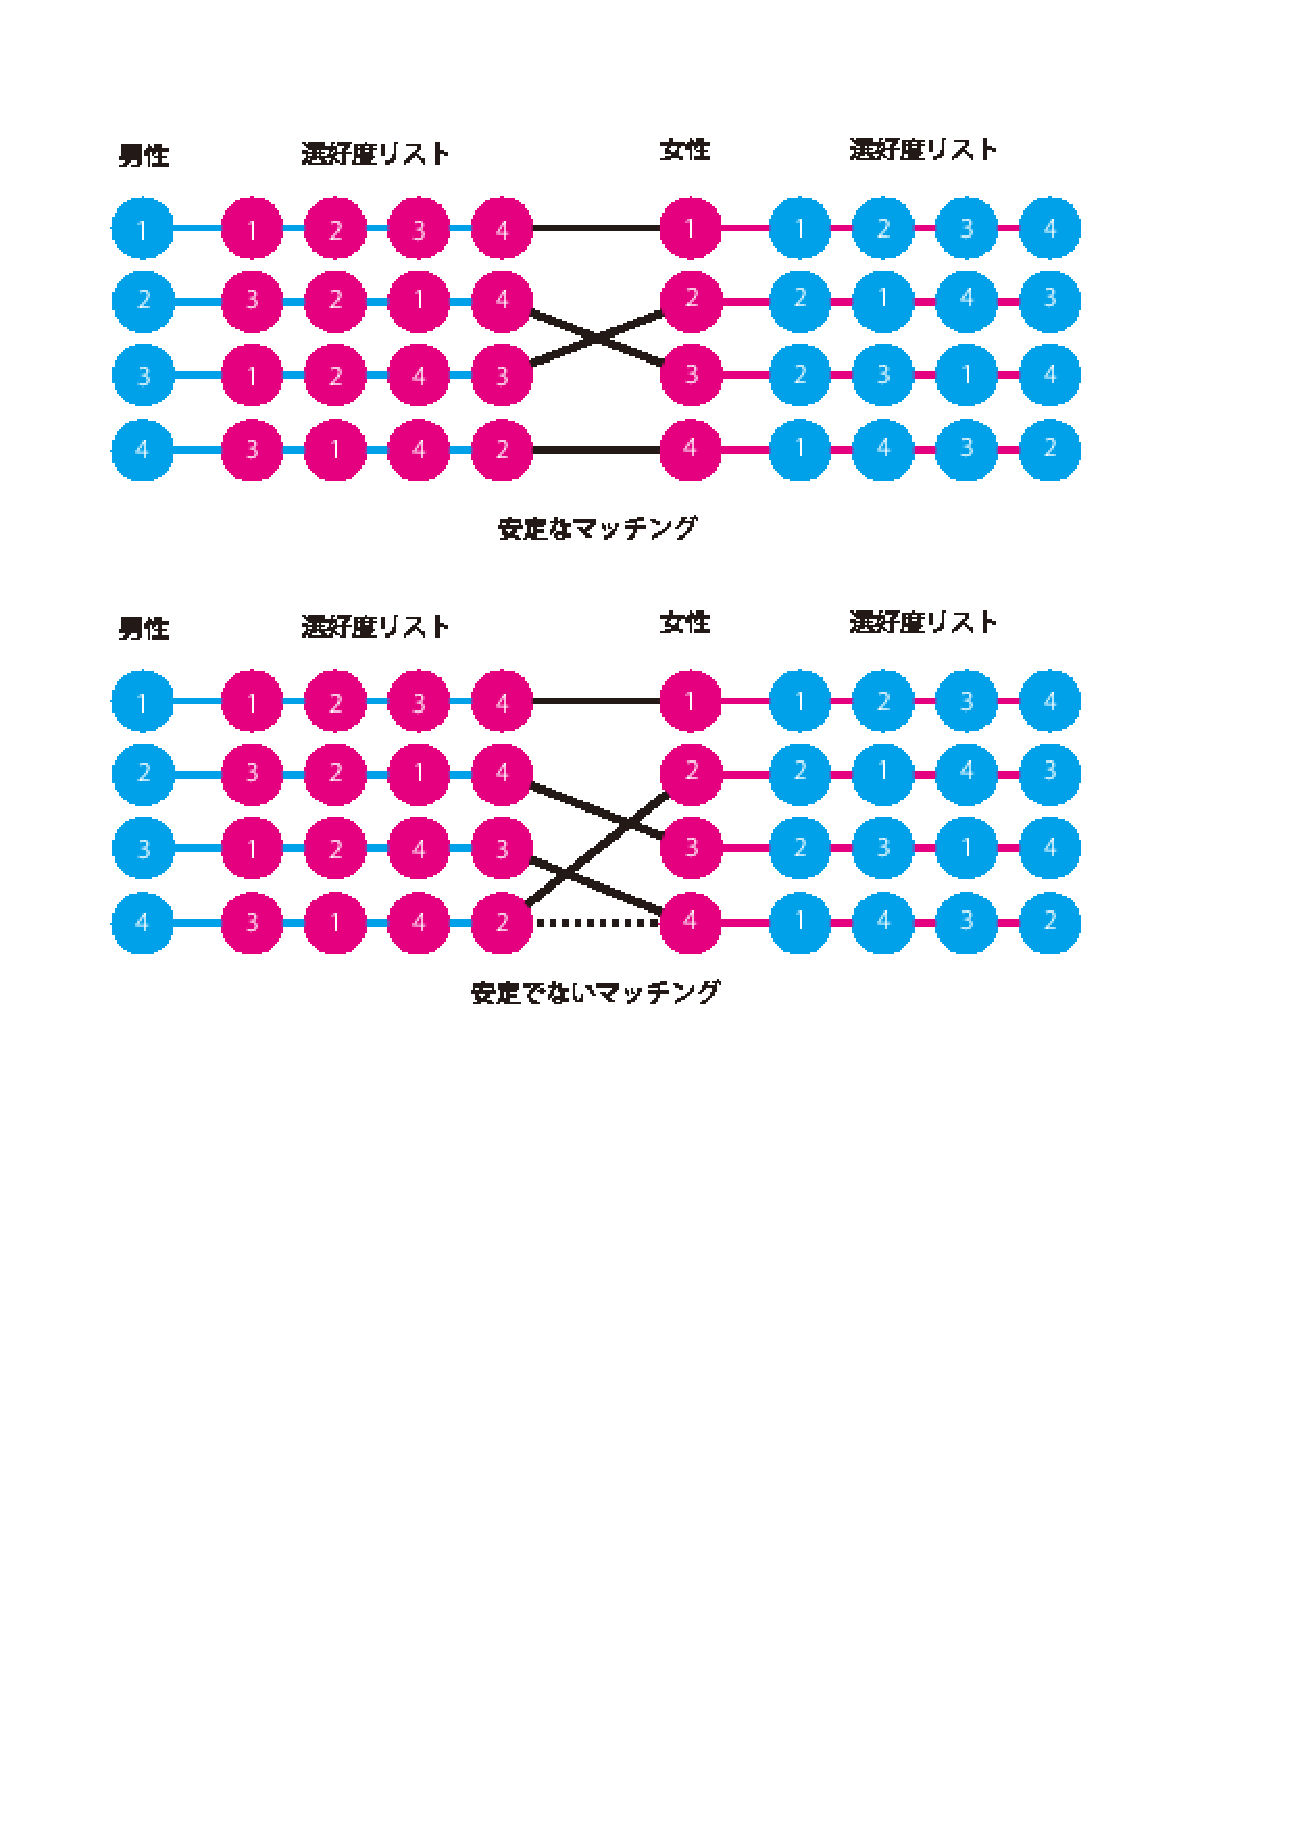
\includegraphics[scale=0.5]{image/match.eps}
  \end{center}
  \caption{安定結婚問題の例}
  \label{match}
\end{figure}

安定結婚問題の全ての事例に対して, 安定なマッチングが必ず存在することが証明されている.
\def\gsa{Gale-Shapleyアルゴリズム}
そのようなマッチングを見つける手法として, \gsa というものが知られている.
\gsa の疑似コードを以下に示す

% \begin{figure}
\lstinputlisting[label=Gale-Shaplay]{src/gale_shapley.py}
% \caption{Gale-Sharpleyアルゴリズム}
% \end{figure}

上記アルゴリズムが終了した際に得られるマッチングは安定である.
証明の概略を以下に示す.

以下, 便宜的に, xがyよりzを好むことを$y <_x z$と表す.

\begin{proof}
\gsa で得られたマッチングが安定であることの証明

得られたマッチングが安定ではないと仮定する.

すなわち, 二つのペア$(m_1, f_1), (m_2, f_2)$のブロッキングペア$(m_1, f_2)$が存在して, $f_1 <_{m_1} f_2 \land m_1 >_{f_2}m_2$であると仮定する.

(i) 男性$m_1$は好きな順番に女性にプロポーズをしている. $f_1 <_{m_1} f_2$より, $m_1$は$f_2$にすでにプロポーズをしている.

(ii) また, 女性は相手を変える際には, より選好度の高い男性にしか変えない. (i)より$f_1$はすでに$m_1$にプロポーズされているので, $m_1 <_{f_1} m_2$である.

これは仮定の$m_1 >_{f_2}m_2$に矛盾するので, 背理法より得られたマッチングは安定である.

\end{proof}

また,
\begin{enumerate}
\item 一人の男性は同じ女性に二度以上プロポースをしない
\item 女性は婚約すると独身に戻らない
\item 女性はプロポーズされる際その相手が悪くなる事はない
\end{enumerate}

ということから, \gsa は有限回数で終了することが言える. さらに, \gsa は$O(N^2)$時間で終了することが知られている.

上記の説明 では, 便宜上男性が女性に順番に求婚していくという形式をとったが, 女性が男性に順番に求婚していくように置き換える事も可能である.
男性が女性に順番に求婚していき, 最終的に得られるマッチングを男性最良安定マッチングと呼び, 女性が男性に順番に結婚していき最終的に得られるマッチングを女性最良安定マッチングと呼ぶ.

\subsubsection{一対多型安定結婚問題}
この節では, 安定結婚問題の拡張である, 一対多型安定結婚問題について説明する.
本研究ではTweetとニュース断片のマッチングを安定結婚問題として定式化することでアラインメントをとるが, 一般にTweetとニュース断片の数は異なるため, \gsa を適用することが出来ない.
一つのニュース断片に複数のTweetが結びつく場合もあるし, 逆に一つもTweetが結びつかない場合も想定される.

このような問題を「一対多型安定結婚問題」として定式化することを考える.

一対多型安定結婚問題に関する選考研究\cite{psmp}では, 一対多型安定結婚問題を定式化している. その概要を以下に示す.

\begin{definittion}
\label{psmp_def_1}
解の定義

男性の集合$M$, 女性の集合$F$, そして各々の女性$f(\in F)$に対する定員(capacity)と呼ばれる非負整数$c_f(f \in F)$が与えられている. このとき, 写像 $\phi : M \rightarrow F$のうち,

\begin{equation}
| \phi^{-1} | \leq c_f, \forall f \in F
\end{equation}

となるものを一対多型結婚問題の解(solution), あるいは縁組と呼ぶ.
\end{definittion}

また, 一対多型結婚問題における安定性を以下のように定義している.

\begin{definittion}
\label{psmp_def_2}
安定性の定義

以下の条件(i)と(ii)を同時に満足する$m \in M$ と $f \in F$の組を, 不安定組(unstable couple)と呼ぶ.

\begin{align}
(i) &\  \exists n \in \phi ^{-1} (f); n <_f m \\
(ii) &\  \phi(m) <_m f
\end{align}

不安定組が存在するとき, 縁組み$\phi: M \rightarrow F$は不安定(unstable)であると言い, そうでないとき, 安定(stable)であるという.
\end{definittion}

ここで, 男性$m \in M$の女性に対する選好を全順序集合$(F, \leq _m)$で表現し, 同様に女性$f \in F$の男性に対する選好を全順序集合$(M, \leq _f)$で表現する.

上で定義されている不安定組は, 安定結婚問題のブロッキングペアに相当するものである.

一対多型結婚問題における安定な縁組みを見つける問題を一対多型安定結婚問題と呼ぶ. この問題をTweetとニュース断片に適用することでTweetとニュース断片のアラインメントをとる.

一対多型の安定結婚問題に置ける選好度リストの例を表\ref{psmp_table}に示す.
また, 表\ref{psmp_table}の選好度リストのもとでの一対多型安定結婚問題の解の例を図\ref{result_of_psmp}に示す.

\begin{table}
\begin{center}
\caption{一対多型安定結婚問題における選好度リストの例}
\label{psmp_table}
\begin{tabular}[t]{|c||c|c|c|c|}
\hline
男性ID & \multicolumn{4}{|c|}{選好度リスト} \\ \hline \hline
1 & 1 & 4 & 3 & 2 \\ \hline
2 & 4 & 2 & 1 & 3 \\ \hline
3 & 4 & 2 & 1 & 3 \\ \hline
4 & 3 & 4 & 2 & 1 \\ \hline
5 & 3 & 2 & 4 & 1 \\ \hline
6 & 3 & 2 & 4 & 1 \\ \hline
7 & 4 & 1 & 3 & 2 \\ \hline
8 & 2 & 3 & 4 & 1 \\ \hline
\end{tabular}
\begin{tabular}[t]{|c||c|c|c|c|c|c|c|c|}
\hline
女性ID & \multicolumn{8}{|c|}{選好度リスト} \\ \hline \hline
1 & 8 & 1 & 5 & 6 & 4 & 2 & 7 & 3 \\ \hline
2 & 3 & 1 & 8 & 2 & 7 & 6 & 5 & 4 \\ \hline
3 & 2 & 1 & 7 & 4 & 5 & 3 & 8 & 6 \\ \hline
4 & 5 & 8 & 3 & 1 & 2 & 6 & 4 & 7 \\ \hline
\end{tabular}
\end{center}
\end{table}

\begin{figure}
  \begin{center}
    \includegraphics[scale = 0.5]{image/psmp.eps}
  \end{center}
  \caption{一対多型安定結婚問題の結果の例}
  \label{result_of_psmp}
\end{figure}

ここで, 便宜的にIDがnの男性を$m_n$, IDがnの女性を$f_n$と表す.

図\ref{result_of_psmp}の右側の例は, 全ての組み合わせが定義\ref{psmp_def_2}の安定性の条件を満たしているので, 安定な解であると言える.
それに対して, 左側の例では, 組み合わせ$(m_3, f_4)$について,

\begin{align}
(i)  & \ m_7 \in \phi^{-1} (f_4) \land m_7 < m_3   \\
(ii) & \ f_2(= \phi(m_3)) < _{m_3} f_4
\end{align}

が成り立ち, $(m_3, f_4)$は不安定組となる.

先に挙げた選好研究\cite{psmp}では, \gsa を拡張することで一対多型安定結婚問題の解を導いている.
そのアルゴリズムの概要を以下に示す.

\lstinputlisting[label=Gale-Shaplay]{src/psmp.py}

上記のアルゴリズムにより, 男性の集合$M$, 女性の集合$F$に対して$O(|F| \cdot |M| \cdot log(|M|))$の時間計算量で一対多型の安定結婚アルゴリズムを解くことができる.

\subsection{形態素解析}
本研究の最終的な目的は, 言語に依存しないツールの構築であるが, 実験段階では便宜的に日本語を対象とする. 日本語は, 英語等の言語と違い, 単語間の区切りの位置が明確でない. そのため, どの文字からどの文字が一つの単語であるのかを分析する必要がある. 今回は, MeCab\cite{MeCab}という形態素解析ツールを使う. MeCabは, Conditional Random Fieldsを用いて日本語の単語区切りと, それぞれの単語の品詞を推定するツールである. 例えば, 「東京都に住む」という文章は, 「東京 都 に 住む」という区切り方に分割され, 「東京」は名詞, 「都」は接尾辞, 「に」は格助詞, 「住む」は動詞であると, 品詞が解析される.

% 一般に, 格助詞や助動詞は機能語であるので, 文章の特性を調べる際には重要でない. その一方, 名詞, 動詞, 形容詞は内容語になりやすい傾向にある. 本研究では, 機能語である格助詞, 助動詞等の機能語の除去をMeCabでの形態素解析の段階で行う. 対象言語を広げる場合には, 機能語の除去のための代替の手段を考える必要がある.

\section{実験}
\def\googlenews{Google\_news\_jp}
\subsection{概要}

本研究では
\begin{itemize}
\item 実験A:tf-idfによる内容語の抽出
\item 実験B:tweetとニュース断片の関連度の計算
\item 実験C:tweetとニュース断片のアラインメント
\end{itemize}
の三つの実験を行った.

実験Aでは, tf-idfによりインターネット上のニュース記事とtwitterの書き込みから内容語を抽出するシステムを構築し, その性能を評価した.
内容語の抽出に関しては, サンプル記事と, その記事に言及しているtweetに現れている各単語についてtf-idfを計算し, ソートすることにより, 内容語と判定する基準である閾値がどのような値になるのかを検討した.

実験Bでは, ニュース記事とtweetの間の関連度を「一致する単語」, 「言い換えの単語」, 「類似の関係にある単語」を指標として計算し, 人間の手によって評価された関連度と比較することでその性能を評価した.

実験Cでは, 実験Bで評価したニュース記事とtweetの関連度の計算手法をもとに, ニュース記事とtweetの間のアラインメントを安定結婚アルゴリズムにより計算した.
このアラインメントの結果も, 人間の手によって生成されたアラインメントと比較することでその性能を評価した.

実験Cの評価の結果, あまり人手によるアラインメントとの一致度が高くなかったため, アルゴリズムを改良した上で追実験を行った. 追実験に関しては\ref{additional_expr}にて詳しく説明する.

\subsection{実験条件}
\subsubsection{実験サンプル}
本研究ではサンプルとして, Twitter上のアカウント"@\googlenews "によって取り上げられているニュースを使用した.
"@\googlenews" は, 様々な報道機関が提供しているインターネット上の記事のタイトル・URLを紹介しているアカウントである.

本研究では, 収集したニュース記事のタイトルを本文中に含むtweetをその記事に言及するtweetとみなし使用する. ただし, "@Google\_news\_jp"のような単なるニュース紹介のアカウントのtweetは, 個人の意見や感想を含まないために除外する. 記事に言及するtweetは記事のタイトルやURLを内部に含む場合が多いので, その部分はtweetの本文から除外して分析をする.

tf-idfにおいてidfを計算するためのデータセットとしては, "@Google\_news\_jp"のニュース記事から20記事を集めた物を使用する.

また, ニュース断片とTweetの関連度の評価, ニュース断片とTweetのアラインメントの計算のためのニュース記事のサンプルは, 2014年12月1日から2014
年12月31日の間のニュースの中で, 多くのTweetに言及されているものを10記事選択して取り扱った. 本研究で取り扱ったニュース記事のタイトルを表\ref{news_table}に示す.

\begin{table}
\begin{center}
\caption{本研究で取り扱ったニュース記事の一覧}
\label{news_table}
\begin{tabular}[t]{|c||l|}
  \hline
  記事ID & タイトル \\
  \hline
  \hline
1 & 救助中ヘリから落下, 心肺停止の1人を翌日発見 \\ \hline
2 & 石破氏なお秘密報道に疑問 「処罰対象ではないが…」 \\ \hline
3 & レーシック手術の被害情報5年で80件, 目の痛みや矯正のしすぎ/消費者庁 \\ \hline
4 & 秘密法案, 与党が夜にも成立強行 会期2日延長, 攻防は最終局面 \\ \hline
5 & 人類最古のDNA抽出…40万年前の人骨から \\ \hline
6 & 「ふなっしー」酷似「きゃべっしー」に苦情殺到 \\ \hline
7 & 甘利氏が治療でTPP会合欠席へ 早期の舌がん, 一時辞意も慰留 \\ \hline
8 & 自殺原因は過大なノルマ・罵声…日本郵便を提訴 \\ \hline
9 & 軽自動車保有税上げ 平均数千円, 15年10月までに \\ \hline
10 & 米中会談は5時間半, 防空圏「認めない」と副大統領, 「日中ホットライン確立を」 \\ \hline
\end{tabular}
\end{center}
\end{table}

\subsubsection{人手によるアラインメント}
\label{align_by_human}

本実験では, 作成したツールの精度の評価のために, 15人の被験者に実験に参加してもらい, 人手によるTweetとNews断片のアラインメントのサンプルの収集を行った.
本研究では, 以下の二つの実験を行った.
\begin{itemize}
  \item 実験I: 人手によるTweetとNews断片の関連度の評価
  \item 実験II: 人手によるTweetのNews断片への結びつけ(アラインメント)
\end{itemize}

実験Iでは, 最初に被験者に記事のタイトルと全文を提示する.
その後, 一つの記事の断片と10のTweetを被験者に見せ, それぞれのTweetが提示されているニュース断片とどのくらいの関連度があるのかを四段階で判定してもらった.
関連度の程度に関しては,
一段階目を「ほとんど関連していない」,
二段階目を「あまり関連していない」,
三段階目を「やや関連している」,
四段階目を「強く関連している」とした.
この判定をニュース中のすべてのニュース記事断片について行ってもらった.
関連度の評価尺度はTweetとNews断片中に含まれる単語をもとに判断するようにあらかじめ指示しておいた.
実験Iの実験インターフェースの概要を図\ref{annotation_by_human_A}に示す.

\begin{figure}[t]
  \begin{center}
    \fbox{
      \includegraphics[scale = 0.3]{image/annotation_by_human_A.eps}
    }
  \end{center}
  \label{annotation_by_human_A}
  \caption{実験Iのインターフェース}
\end{figure}

実験IIでも, 最初に被験者に記事のタイトルと全文を提示する.
その後, 一つのTweetと, 記事の断片すべてを見せ, 提示したTweetがどの記事断片と結びつけるかをYESかNOかで応えてもらった.
この判定をそのニュースに言及している40のTweetについて行ってもらった.
結びつけの判定は実験Iと同じくTweetと記事断片中に含まれる単語をもとに判断するようにあらかじめ指示しておいた.
また, 一つのTweetが複数の記事断片と繋がるような場合も許容し, 反対にどの記事断片とも結びつかないようなTweetが存在する場合も許容するようにした.
一つのTweetが複数の記事断片と繋がり場合は, 多くても2~3個の記事断片に留めるようにあらかじめ指示しておいた.
これは, ほとんどの記事断片と繋がってしまうようなTweetが現れるのを事前に防ぐためである.

実験IIの実験インターフェースの概要を図\ref{annotation_by_human_B}に示す.

\begin{figure}[t]
  \begin{center}
    \fbox{
      \includegraphics[scale = 0.3]{image/annotation_by_human_B.eps}
    }
  \end{center}
  \label{annotation_by_human_B}
  \caption{実験IIのインターフェース}
\end{figure}

\subsubsection{評価尺度}
\def\kappac{$\kappa$係数}

人手による関連度評価やアラインメントの結果は, \kappac\cite{kappa}により評価した. \kappac は, 人手によるクラス分類の際の, 個人ごとによるずれを評価する尺度である. 二人の異なる分類者の間で, \kappac は以下の式によって定義される.

\begin{equation}
\kappa = \frac{Pr(a) - Pr(e)}{1 - Pr(e)}
\end{equation}

ここで, $Pr(a)$は実際に観測された一致率である. それに対して, $Pr(e)$は二人のクラス分類が偶然一致する確率である.
上記のように定義することで, \kappac では, 偶然の要素を除いた二者の一致度合いを測定することが出来る.

\begin{table}
\begin{center}
\caption{二者によるクラス分類の例}
\label{classifi_2}
\begin{tabular}[t]{|c|c|c|c|}
  \hline
  \multirow{2}{*}{} & & \multicolumn{2}{|c|}{B} \\ \hline
                           &  & Yes & No \\ \hline
  \multirow{2}{*}{A} & Yes    & 20  &  5   \\ \cline{2-4}
                     & No     & 10  & 15  \\ \hline
\end{tabular}
\end{center}
\end{table}

分類者Aと分類者Bによる, 二値のクラス分類の例を表\ref{classifi_2}に示す.
この例では, 全体の一致率は
\begin{equation}
\frac{20 + 15}{20 + 5 + 10 + 15} = 0.7
\end{equation}
より, 0.7である.
一方, 分類者AがYesに分類する確率$P_{A,yes}$, Noに分類する確率$P_{A,no}$, 分類者BがYesに分類する確率$P_{B, yes}$, Noに分類する確率$P_{B, no}$はそれぞれ以下のように求めることができる.

\begin{eqnarray}
P_{A,yes} = \frac{20 +  5}{20 + 5 + 10 + 15} = 0.5\\
P_{A,no}  = \frac{10 + 15}{20 + 5 + 10 + 15} = 0.5\\
P_{B,yes} = \frac{20 + 10}{20 + 5 + 10 + 15} = 0.6\\
P_{B,no}  = \frac{ 5 + 15}{20 + 5 + 10 + 15} = 0.4
\end{eqnarray}

したがって, 両方の分類者が「偶然」同時にyesに分類する確率は$P_{A,yes}*P_{B,yes}$, 両方の分類者が同時にnoに分類する確率は$P_{A,no}*P_{B,no}$で表すことができ, 両者の分類結果が偶然一致する結果$Pr_{e}$は以下のように求まる.

\begin{equation}
Pr_{e} = P_{A,yes}*P_{B,yes} + P_{A,no}*P_{B,no} = 0.5
\end{equation}

以上より, この例に置ける分類者Aと分類者Bの間の\kappac は
\begin{equation}
\kappa = \frac{0.7 - 0.5}{1 - 0.5} = 0.4
\end{equation}
となる.

\kappac の値の目安を表\ref{kappa_standard}に示す. 一般に二人の分類者の一致度合いは, \kappac が0であれば一致なし(偶然と同程度の一致), 0から0.4の間であれば弱い一致(Poor), \kappac が0.4から0.6の間であればそこそこの一致(Moderate), \kappac が0.6から0.8の間であれば良い一致(Good), \kappac が0.8から1の間であれば非常に高い一致度(Excellent)であるとみなされる.

\begin{table}
\begin{center}
\caption{\kappac の目安}
\label{kappa_standard}
\begin{tabular}[t]{|c|c|}
  \hline
  \kappac & 評価 \\ \hline \hline
  0.8 - 1.0 & Excellent \\ \hline
  0.6 - 0.8 & Good \\ \hline
  0.4 - 0.6 & Moderate \\ \hline
  0.0 - 0.4 & Poor \\ \hline
\end{tabular}
\end{center}
\end{table}

多段階のクラス分類の場合, 上記の定義の通りに\kappac を計算すると, クラス数が多くなるほど二者の分類結果が一致する確率が低くなってしまうので, \kappac を多段階クラス用に拡張した重み付け\kappac を使用する. 重み付け\kappac では, $Pr(a)$は以下の式で求められる.
\begin{equation}
Pr(a) = \frac{1}{N} \sum _{i=1} ^{k} \sum _{i=j} ^{k} w_{i,j} x_{i, j}
\end{equation}

ここで, $N$は全サンプル数, $k$はクラス数, $i, j$はクラスのID, $x_{i, j}$は片方の分類者がクラス$i$に分類し, もう片方の分類者がクラス$j$に分類したサンプルの総数である.
$w_{i, j}$は, 重み付け係数で, 以下により定義される.

\begin{equation}
w_{i, j} = 1 - \frac{(i - j)^2}{(k-1)^2}
\end{equation}

多段階のクラス分類の例を表\ref{classifi_4}に示す.
この例では, A, Bの二人の分類者が与えられたサンプルをGrade1からGrade4の4段階のクラスに分類している.

\begin{table}
\begin{center}
\caption{二者による多段階クラス分類の例}
\label{classifi_4}
\begin{tabular}[t]{|c|c|c|c|c|c|}
  \hline
  \multirow{2}{*}{} & & \multicolumn{4}{|c|}{B} \\ \hline
                            &   & Grade 1 & Grade 2 & Grade 3 & Grade 4 \\ \hline
  \multirow{4}{*}{A} & Grade 1  & 20 &  6 &  3 &  2   \\ \cline{2-6}
                     & Grade 2  &  5 & 20 &  2 &  3   \\ \cline{2-6}
                     & Grade 3  &  2 &  6 & 10 &  2   \\ \cline{2-6}
                     & Grade 4  &  4 &  2 &  3 &  10   \\ \hline
\end{tabular}
\end{center}
\end{table}

重み付けをしない場合の多段階クラス分類では, $Pr(a) = 0.6, Pr(e) = 0.27$より \kappac は

\begin{equation}
  \kappa = \frac{0.6 - 0.27}{1 - 0.27} = 0.24
\end{equation}

となり, 分類者Aと分類者Bの間の一致度はかなり低いと判定される.

一方, 重み付けをした場合の多段階クラス分類では, $Pr(a) = 0.89, Pr(e) = 0.27$より \kappac は

\begin{equation}
  \kappa = \frac{0.89 - 0.27}{1 - 0.27} = 0.51
\end{equation}

となり, 分類者Aと分類者Bの間の一致度はそこそこ高いと判定される.

このように, 二人の分類者のクラス分類が一致しなかった場合も, 一致するクラスと近い場合は「惜しい例」として, 重み付けをされた上で$Pr(a)$に加算されるので, 重み付け \kappac では多段階のクラス分類で \kappac が極端に低く見積もられる問題に対処することができる.
なお, 重み付け\kappac で$k=2$とした場合は重み付けをしなかった場合の\kappac と完全に一致する.


本研究では, Twitter上の投稿とニュース断片の関連度の計算を4段階の多段階クラス分類, Twitter上の投稿とニュース断片のアラインメントを, 結びつけるか結びつけないかの二値のクラス分類としてモデル化し, \kappac を適用することでその結果を評価する.

% アラインメントの結果の評価は, precision-recall\ref{information}を尺度に行う.
% precisionとrecallは検索エンジンの性能評価などに用いられる評価尺度で, 以下の式によって表される.

% \begin{align}
%   {\rm precision} &= \frac{R}{N}\\
%   {\rm recall} &= \frac{R}{C}
% \end{align}
%   ここで, $N$はアラインメントした結果webニュースの断片に対応づけられたtweetの数, $C$は正解データでwebニュースの断片に対応づけられるべきとされたtweetの数, $R$はアラインメントした結果webニュースの断片と対応づけられ, なおかつ正解とも一致したtweetの数である. これらの値を合わせたF-scoreで, アラインメントの評価を行う. F-scoreはprecisionとrecallの調和平均であり, 以下の式によってあらわされる.

% \begin{align}
%   F &= \frac{2}{\frac{1}{\rm precision} + \frac{1}{\rm recall}} \\
%     &= \frac{2R}{N+C}
% \end{align}

\subsubsection{改良アルゴリズムによるアラインメント}
\label{additional_expr}

実験Cの結果, 本研究で作成したツールによるTweetとニュース断片のアラインメントと, 人手による, アラインメントはほとんど一致しなかった. これは, 安定結婚問題における, 一つのニュース断片にいくつのTweetが関連づけられるかのパラメータである$c$(capacity)を定数

\begin{equation}
  c = \frac{ |\bf{Tweets}| }{ |\bf{Sentences}| }
\end{equation}

にしていたのが原因と考えた.
ここで, $\bf{Tweets}$はそのニュースに言及しているTweetの集合, $\bf{Sentences}$はそのニュースを分割した断片の集合である.

本来, どのくらいのTweetがニュース断片に結びつくかは, そのニュース断片のもつ素性に依存するべきである.
そこで, 追実験ではどのくらいのTweetがニュース断片に結びつくかを決定づける素性をそのニュース断片のtf-idf値の総和であると仮定し,
安定結婚問題における$c$を以下のように定義し直した.

\begin{equation}
  c_{s} =  |\bf{Tweets}| \frac{\sum _{w \in s} \bf{tfidf}_{News}(w)}{\sum _{s' \in \bf{Sentences}} \sum _{w \in s'} \bf{tfidf}_{News}(w)}
\end{equation}

ここで, $c_s$はニュース断片$s$にどれだけのTweetが結びつくことができるかの容量, $\bf{tfidf}_{News}(w)$は, あるNewsにおける単語wのtf-idf値を表す.

以上の条件のもと追実験を行いその性能を評価した.

\subsection{実験結果}
\subsubsection{内容語の抽出}

いくつかのニュース記事に対して, その中に出現する全ての単語のtf-idfを計算し, その値を降順にソートして並べた結果を図\ref{content_word}に示す.

\begin{figure}[htbp]
  \begin{center}
    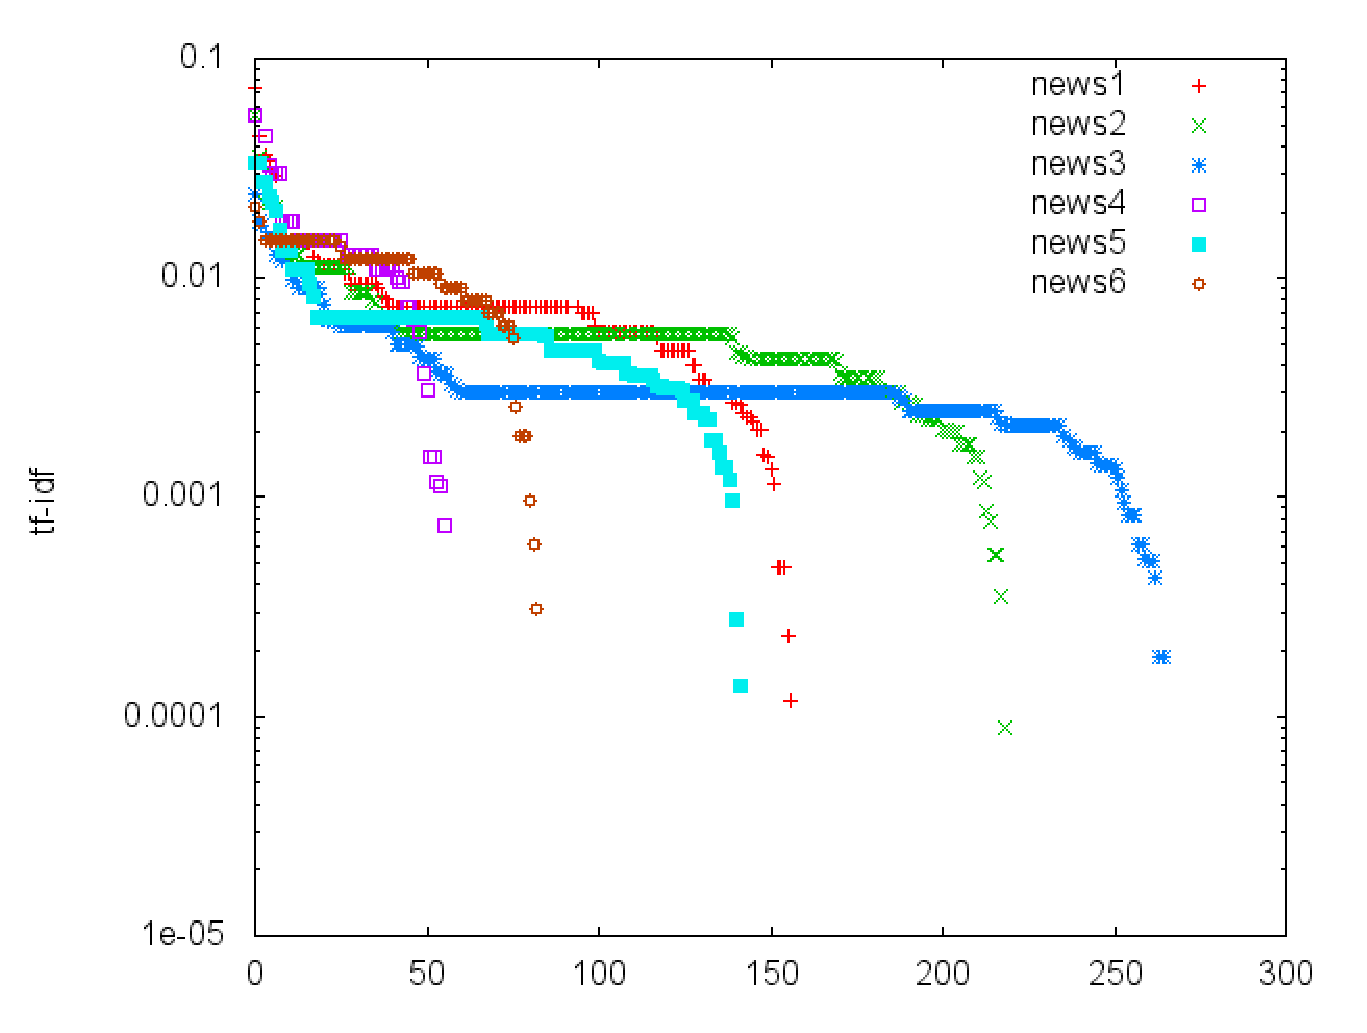
\includegraphics[scale = 0.5]{image/content_word.eps}
  \end{center}
  \label{content_word}
  \caption{tf-idfの計算結果}

\end{figure}

図\ref{content_word}のように, tf-idfの分布が三つの集団に分かれる結果となった. 一つは, 一番左側のtf-idfが極端に高い単語群である. これは, いわゆるキーワードであると言える. 実際, コーヒーの健康への影響を題材にした記事では, 「コーヒー」「杯」といった単語がこの集団に属していた. 二つ目は, 中央部の平らな, 平均的なtf-idfをもつ集団である. コーヒーを題材にした記事では, 「カフェイン」や「サウスカロライナ」などの内容語が多く所属していたのに対し, 「ただし」「よう」等のあまり情報を含まない単語も所属していることが確認された. 三つ目は, 右側で急降下している, 低いtf-idfをもつ集団である. この集団には「て」「に」「を」「は」などの助詞を含む機能語が多く所属していた.

\subsubsection{Tweetとニュース記事断片の関連度測定}
本研究では\ref{align_by_human}で述べたように, 人手によるTweetとニュース記事断片の関連度の測定を行った.
得られた測定結果から \kappac を測定した結果を表\ref{kappa_human_A}に示す.

\kappac の測定測定は, ニュース記事のうち2人以上の被験者により関連度の測定を行われたものについてのみ行った.

\begin{table}
\begin{center}
\caption{Tweetとニュース断片の関連度測定における被験者間での \kappac}
\label{kappa_human_A}
\begin{tabular}[t]{|c||l|c|}
  \hline
  記事ID & タイトル & \kappac\\
  \hline
  \hline
1 & 救助中ヘリから落下, 心肺停止の1人を翌日発見 & 0.75 \\ \hline
2 & 石破氏なお秘密報道に疑問 「処罰対象ではないが…」 & 0.69 \\ \hline
3 & レーシック手術の被害情報5年で80件, 目の痛みや矯正のしすぎ/消費者庁 & 0.74 \\ \hline
4 & 秘密法案, 与党が夜にも成立強行 会期2日延長, 攻防は最終局面 & 0.73 \\ \hline
6 & 「ふなっしー」酷似「きゃべっしー」に苦情殺到 & 0.70 \\ \hline
8 & 自殺原因は過大なノルマ・罵声…日本郵便を提訴 & 0.88 \\ \hline
\end{tabular}
\end{center}
\end{table}

\kappac はおよそ0.7から0.9の間の値になった. このことから人手によるTweetとニュース記事断片の間の関連度測定は, 被験者間で高めの一致をしていると言える.

次に, 本研究で制作したツールによるTweetとニュース記事断片の関連度を測定し, その結果と人の手による関連度測定の結果との間で\kappac を測定した. 結果を\ref{kappa_auto_A}に示す. なお, 一つの記事を複数の人間で評価していた場合は, 平均をとって掲載している. 比較用に人同士での\kappac の値を併記しておく.

\begin{table}
\begin{center}
\caption{Tweetとニュース断片の関連度測定における本研究で制作したツールと被験者の間での \kappac}
\label{kappa_auto_A}
\begin{tabular}[t]{|c||c|c|}
  \hline
  記事ID & ツール-人の\kappac & 人-人の\kappac\\
  \hline
  \hline
  1 & 0.69 & 0.75 \\ \hline
  2 & 0.74 & 0.69 \\ \hline
  3 & 0.72 & 0.74 \\ \hline
  4 & 0.78 & 0.73 \\ \hline
  5 & 0.81 & 未測定 \\ \hline
  6 & 0.76 & 0.70 \\ \hline
  7 & 0.71 & 未測定 \\ \hline
  8 & 0.85 & 0.88 \\ \hline
  9 & 0.69 & 未測定 \\ \hline
\end{tabular}
\end{center}
\end{table}

こちらの\kappac もおよそ0.7から0.9の間の値となった. このことから, 本研究で制作したツールによるTweetとニュース記事断片の間の関連度測定は人手によるものと同程度の精度を達成しているということが言える.

\subsubsection{Tweetのニュース記事断片へのアラインメント}
次に, 人手によるTweetとニュース記事断片の結びつけ(アラインメント
)の測定を行った. 得られた測定結果から\kappac を測定し結果を表\ref{kappa_human_B}に示す.

\begin{table}
\begin{center}
\caption{Tweetとニュース断片のアラインメントにおける被験者間での \kappac}
\label{kappa_human_B}
\begin{tabular}[t]{|c||l|c|}
  \hline
  記事ID & タイトル & \kappac\\
  \hline
  \hline
  1 & 救助中ヘリから落下, 心肺停止の1人を翌日発見 & 0.21 \\ \hline
  2 & 石破氏なお秘密報道に疑問 「処罰対象ではないが…」 & 0.20 \\ \hline
  4 & 秘密法案, 与党が夜にも成立強行 会期2日延長, 攻防は最終局面 & 0.20 \\ \hline
  6 & 「ふなっしー」酷似「きゃべっしー」に苦情殺到 & 0.30 \\ \hline
  8 & 自殺原因は過大なノルマ・罵声…日本郵便を提訴 & 0.36 \\ \hline
\end{tabular}
\end{center}
\end{table}

\kappac は0.2から0.4の間の値となった. この事から人手によるTweetとニュース記事断片のアラインメントの測定者間の一致の度合いは, それほど高くないということが言える.

次に, 本研究で制作したツールによりTweetとニュース記事断片のアラインメントを作成し, その結果と人の手によるアラインメントの結果との間で\kappac を測定した. 結果を表\ref{kappa_auto_B}に示す. 比較用に人同士での\kappac の値を併記しておく.

\begin{table}
\begin{center}
\caption{Tweetとニュース断片のアラインメント作成における本研究で制作したツールと人の間での \kappac}
\label{kappa_auto_B}
\begin{tabular}[t]{|c||c|c|}
  \hline
  記事ID & ツール-人の\kappac & 人-人の\kappac\\
  \hline
  \hline
  1 & -0.030 & 0.21 \\ \hline
  2 &  0.001 & 0.20 \\ \hline
  3 & -0.043 & 未測定 \\ \hline
  4 & -0.012 & 0.20 \\ \hline
  5 &  0.131 & 未測定 \\ \hline
  6 & -0.042 & 0.30 \\ \hline
  7 & -0.006 & 未測定 \\ \hline
  8 & -0.014 & 0.36 \\ \hline
  9 & -0.003 & 未測定 \\ \hline
\end{tabular}
\end{center}
\end{table}

\kappac は0の近傍の値になった.
このことから, 人手によるTweetとニュース記事断片のアラインメントの結果と, 本研究で制作したツールによるアラインメントの結果の一致度はランダムにアラインメントを行った場合に等しいということが言える.

実験結果が良くなかったため, アルゴリズムの改良(\ref{additional_expr}節参照)を施し, 同様の評価を行った. 結果を表\ref{additional_kappa_auto_B}に示す. 今回の改良では, 一致度の向上は見られなかったが, アラインメントの結果はより直感に即したものになった.

\begin{table}[hb]
\begin{center}
\caption{Tweetとニュース断片のアラインメント作成における改良したツールと人の間での \kappac}
\label{additional_kappa_auto_B}
\begin{tabular}[t]{|c||c|c|c|}
  \hline
  記事ID & 改良したツール-人の\kappac & 元のツール-人の\kappac & 人-人の\kappac\\
  \hline
  \hline
    1 & -0.0159 & -0.030 & 0.21 \\ \hline
    2 & -0.0141 &  0.001 & 0.20 \\ \hline
    3 &  0.0617 & -0.043 & 未測定 \\ \hline
    4 & -0.0204 & -0.012 & 0.20 \\ \hline
    5 & -0.0331 &  0.131 & 未測定 \\ \hline
    6 & -0.0420 & -0.042 & 0.30 \\ \hline
    7 & -0.0290 & -0.006 & 未測定 \\ \hline
    8 & -0.0331 & -0.014 & 0.36 \\ \hline
    9 &  0.0504 & -0.003 & 未測定  \\ \hline
\end{tabular}
\end{center}
\end{table}

\clearpage
\section{考察}
\subsection{内容語の抽出}
内容語の抽出では, 図\ref{content_word}のように値がおおまかに3つの部分に分かれる結果となった. このうち一番tf-idfの低い集団が, 格助詞等の情報を持たない単語の集団であることが確認された. この部分に含まれる単語を除外することで内容語の抽出を行うことができる.
このことにより, 提案手法により対象の文章中から内容語を抽出することが可能であることが確認できた.
真ん中の集団にも情報が持たない単語が紛れ込んでいたが, 本研究の内容語抽出におけるツールとしては十分な精度を発揮していると考える.

\subsection{Tweetとニュース断片の関連度評価}
Tweetとニュース断片の関連度評価では, 本研究で作成したツールによる評価と人手による評価の一致度を比較した.

まず, 実験で収集した人手による評価の間での一致度を測定したが, 表\ref{kappa_human_A}に示すようにかなり高い一致度を得ることができた.
この事から, Tweetとニュース断片がどのくらい関連をしているかを判断するタスクは, 複数人の間で一定の普遍性をもっていると判断することが出来る.
従って, 本研究で作成したツールによるTweetの関連度評価を人手による関連度評価の結果に近づけることには大きな意義があると考えられる.

次に, 機械的にTweetとニュース断片の値を評価するツールを作成し, そのツールによる関連度評価の結果と人手による関連度評価の結果との間の一致度を測定したが, 表\ref{kappa_auto_A}に示すように, 人による関連度評価と非常に一致度の高い結果を得る事ができた.

このことから, 本研究のツールによるTweetとニュース断片の間の関連度評価は人手による関連度評価に近い精度を達成していると考えられる.

\subsection{Tweetのニュース記事断片へのアラインメント}
Tweetとニュース断片の関連度評価では, 本研究で作成したツールによる評価と人手による評価の一致度を比較した.

まず, 実験で収集した人手による評価の間での一致度を測定した. 結果は, 表\ref{kappa_human_B}に示すように0.2から0.3の間の値となった.
これは, \kappac としては低めの値であり, 複数人の間での一致度はあまり高くないと判断される.
このような結果になったのは, そもそもTweetのニュース記事断片へのアラインメントがそもそも難しいタスクであることが原因であると考えられる.
この結果から, 本研究で作成したツールによるアラインメントが, 人手によるアラインメントとの間で0.2から0.3の\kappac を達成できれば, 十分に人間に近い精度を達成していると考えられる.

次に, 機械的にTweetをニュース断片に結びつけるするツールを作成し, そのツールによるアラインメントの結果と人手によるアラインメントの結果との間の一致度を測定した. 残念ながら結果は, 表\ref{kappa_auto_B}に示すように人手によるアラインメントによる0.2から0.3の一致度には遠く及ばない値となった.

この理由は, 安定結婚問題における, 一つのニュース断片にいくつのTweetが関連づけられるかのパラメータである$c$(capacity)を定数にしていたことにあると考えた.

この結果を受けて\ref{additional_expr}節で取り上げた改良を施したが, \ref{additional_kappa_auto_B}に示すように, 一致度に改善は見られなかった.

このような結果になったのは, そもそも人手によるアラインメントの基準と, 本研究のツールによるアラインメントの目標とする基準が異なることが原因であると考える.

本研究の目標は, News記事へのTweetの結びつけによる情報の付与であった.
そのためには, Tweetをニュース断片に結びつける際に一つのニュース断片にほとんどのTweetが結びついてしまうような結果は好ましくないと考えられる.
このような結果を防止するために, どのニュース断片にどれくらいのTweetが結びつく事ができるかをパラメーターによって制御できる安定結婚問題による定式化を採用した.

このような基準が背後にあるために, 単純に関連度の高そうなTweetをニュース断片に結びつけて行った人手によるアラインメントの結果との食い違いが生じたのだと推測される.

% 一方, 人手によるアラインメントでは, ユーザーにTweetとを提示して, その中からニュース断片に結びつきそうなTweetをいくつか選択してもらうという方式をとった.
% 結果, 一つのツイートが多くのニュース断片に結びつけられたり, まったく使用されないTweet例が発生し, これが本研究で作成したツールのアラインメント基準と食い違ったことで, 一致度が大きく低下する要因となったと考える.

以上のように本研究で作成したツールによるアラインメントは, 人手によるアラインメントとの十分な一致度を得る事ができなかった.
しかしながら, そもそも複数人の間でのアラインメントの結果の一致度がそれほど高くなかったこと, そして本研究のツールには人手によるアラインメントでは考慮されない, Tweetの結びつきのニュース断片間での格差のコントロールという基準があることから, 本研究のツールによるアラインメントには人手によるアラインメントとは一致しないながらも, 妥当性があると考える.

\clearpage
\section{今後の課題}
\subsection{WordNetに依存しない言い換え語・類似語の検出}
今回の実験では「言い換えの関係にある語」, 「互いに類似する語」の検出にWordNetを利用した. しかしながら, WordNetは世界で使用されている全ての言語で作成されているわけではなく, 日本語版のWordNetも語彙がまだ少ないのが現状である. また, Twitter等のソーシャルネットワーキングサービスではネットスラングなどの新しい語彙が頻繁に誕生しているという現状もあり, これにもWordNetでは対応することができない. そこで, WordNetに依存せずに, 機械学習的な手法で言い換え語・類似語の検出をすることが望ましいと考えられる. これを実現するための選好研究として, Linの手法\cite{DekangLin}, Latent Spaceでのモデル化\cite{LatentSpace}を挙げた. これらを実装し, 結果を比較検討しながら二つの手法から選択及び組み合わせをして言い換え語・類似語の検出を実現することを, 今後の課題とする.


\section{結論}
本研究では, ソーシャルネットワーキングサービスであるTwitter上の投稿をインターネット上のニュース記事に自動付与するソーシャルアノテーションツールの構築を行った. 要素技術としてWeb上からのニュースに関連するTweetの収集, Tweetとニュース断片の関連度の計算と, その関連度を利用したTweetとニュース断片のアラインメントがあり, 本研究ではではこのうち, 内容語の抽出, 関連度の計算, アラインメントの実装を行った. 内容語の抽出に関しては効果的に情報を持たない語を除外するアルゴリズムを確率することが出来た. Tweetとニュース断片の関連度の測定では, 人手による関連度の測定と同等の精度をえることが出来た. これは大変顕著な成果であると考えられる. Tweetとニュース断片のアラインメントに関しては人手によるアラインメントとの一致は得られなかったが, 安定結婚問題による定式化により, Tweetの結びつき方のニュース断片間での格差の防止という目標は達成することが出来た.

ソーシャルアノテーションツールは, 情報のプロの書き手と一般人の読み手の距離を縮め, また, 難解な情報へのアクセスをより容易にする画期的なツールである. 本研究の成果を通して, 人の情報との関わり方をより豊かにできるものと自負している. そのために, 今後も研究活動により一層尽力して行きたい所存である.

\clearpage
\section{謝辞}
伊庭研究室での卒業研究は1年間という短い時間でしたが, 様々な方にお世話になりました. 伊庭斉志教授, Danushka Bollegala 講師には研究の進め方を始めとして様々な知識をご教授頂きました.
特にDanushka講師には自然言語処理班全体のサポートに加え, アラインメントのアルゴリズムや評価手法について大変貴重なアドバイスを頂きました.
研究室全体をサポートして頂いた石黒さんを始めとした伊庭研究室の先輩方, 同期として共に研究した自然言語処理班の石渡君, 森君, Ari君に感謝します.

\newpage
\pagestyle{empty}
\begin{thebibliography}{9}
  \bibitem {nlpml} 高村大地, 奥村学.言語処理のための機械学習入門(コロナ社), 2010
  \bibitem {tfidf} Gerard Salton. Introduction to Modern Information Retrieval (Mcgraw Hill, Inc.), 1986
  \bibitem {DekangLin} Lin. Automatic Retrieval and Clustering of Similar Words. COLING '98 Proceedings of the 17th international conference on Computational linguistics - Volume 2 Pages 768-774
  \bibitem {LatentSpace} Weiwei Guo, Mona Diab. Modeling Sentences in the Latent Space. ACL '12 Proceedings of the 50th Annual Meeting of the Association for Computational Linguistics: Long Papers - Volume 1
Pages 864-872
  \bibitem {CoClustering} Inderjit S Dhilon, Subramanyam Mallela, Dharmendra S. Modha. Information-Theoretic Co-clustering. KDD '03 Proceedings of the ninth ACM SIGKDD international conference on Knowledge discovery and data mining
Pages 89-98
 \bibitem {MeCab} 工藤 拓, 山本 薫, 松本 裕治. Applying Conditional Random Fields to Japanese Morphologiaical Analysis, 情報処理学会研究報告. 自然言語処理研究会報告 2004, Pages 89-96
 \bibitem {information} Christopher D. Manning, Prabhakar Raghavan and Hinrich Schu"tze: Introduction to Information Retrieval, Cambridge University Press, 2008.
 \bibitem {wordnet-similarity}Ted Pedersen, Siddharth Patwardhan and Jason Michelizzi. WordNet::Similarity - Measuring the Relatedness of Concepts, HLT-NAACL--Demonstrations '04 Demonstration Papers at HLT-NAACL 2004 Pages 38-41
 \bibitem {smp} D.Gale and L.S.Shapley. COLLEGE ADMISSIONS AND THE STABILITY OF MARRIAGE (1962), The American Mathematical Monthly Vol. 69, pp. 9-15.
 \bibitem {psmp} 奥居 哲, 柴田 祥一, 岡田 稔, 川島 信. 安定結婚アルゴリズムに基づく卒業研究配属の事例研究. 社団法人情報処理学会 研究報告kennkyuuhoukoku 2003, pp. 67-72.
 \bibitem {kappa} David M. W. Powers. The Problem with Kappa
\end{thebibliography}
\end{document}

